\PassOptionsToPackage{svgnames}{xcolor}
\documentclass[12pt,a4paper]{article}
\usepackage[utf8x]{inputenc}
\usepackage[portuguese]{babel}
\usepackage[T1]{fontenc}
\usepackage{amsmath, amssymb, amsfonts}
\usepackage{graphicx}
\usepackage{indentfirst}
\usepackage[left=2cm,right=2cm, top=4cm, bottom=2cm]{geometry}
\usepackage[colorlinks=true,allcolors=blue]{hyperref} % links 
\usepackage[table]{xcolor}
\usepackage{booktabs}
\usepackage{enumitem}
\usepackage{paralist}
\usepackage{makecell}
\usepackage{multicol}
\usepackage{multirow}
\usepackage[title]{appendix}
\usepackage{enumitem}
\usepackage{tabularx,ragged2e}
\usepackage[hang,flushmargin, bottom]{footmisc} %retira a identação da%footnote
\usepackage{adjustbox}


% to make myblock
\usepackage{tcolorbox}
\usepackage{lipsum}
\tcbuselibrary{skins,breakable}
\usetikzlibrary{shadings,shadows}

\usepackage{lipsum}
\usepackage{float}
\usepackage{graphicx,eso-pic}
\usepackage{lipsum}



\usepackage{epstopdf}
\epstopdfsetup{outdir=./}


\usepackage{longtable}
\usepackage{caption,setspace}

\captionsetup{skip=0pt}


\AddToShipoutPictureBG{%
  \AtPageUpperLeft{%
    \raisebox{-\height}{\includegraphics[width=20cm, height=3.8cm]{figures/head2.png}}
  }
  %\AtPageLowerLeft{%
   % \makebox[\paperwidth]{\includegraphics[height=1.7cm]{figures/bottom.png}}
  %}
}

%%%%%%%%%%%% setlength

\setlength{\skip\footins}{12mm} %<------------ space between text and footnote
\setlength{\columnsep}{1cm}
\setlength{\parskip}{0pt}



%%%%%%%%%%%% New commands

\newenvironment{myexampleblock}[1]{
    \tcolorbox[
    %noparskip,
    breakable,
    colframe=blue!85!black,
    colback=white,
    title=#1]}
    {\endtcolorbox}


\newcommand{\tri}{$\blacktriangleright \:$}

\usepackage{lmodern}

\makeatletter
\ifcase \@ptsize \relax% 10pt
  \newcommand{\miniscule}{\@setfontsize\miniscule{2}{3}}% \tiny: 5/6
\or% 11pt
  \newcommand{\miniscule}{\@setfontsize\miniscule{4}{5}}% \tiny: 6/7
\or% 12pt
  \newcommand{\miniscule}{\@setfontsize\miniscule{4}{5}}% \tiny: 6/7
\fi
\makeatother


\newcolumntype{P}[1]{>{\centering\arraybackslash}p{#1}} % centralizar elementos da tabela


\graphicspath{{figures/}}


%%%%%%%%%%%%%%%%%%%%%%%%%%%%%%% Start %%%%%%%%%%%%%%%%%%%%%%%%%%%%%%%%%%%%%%%

\begin{document}

\begin{multicols}{2}

\begin{flushleft}
Luciano Nakabashi \\        
Marcos Júnio Ribeiro \\
Francielly Almeida  \\
\end{flushleft}

\begin{flushright}
Pedro Borges \\
Nícolas Volgarine Scaraboto \\
Rafael de Castro Perez \\
\end{flushright}

\end{multicols}

\vspace{0.2cm}


% sections --------------


Usando dados de 2019 calculei as estatísticas descritivas de vários indicadores disponíveis no SNIS. Esses indicadores são de atendimento e tarifas de água e esgoto.


\begin{table}[H] \centering 
	\begin{minipage}{0.7\textwidth}
	
  \caption{Estatísticas descritivas do Índice de atendimento total de água por natureza (em \%)} 
  \label{tab:in055} 
\begin{tabular}{@{\extracolsep{5pt}} cccccc} 
\\[-1.8ex]\hline 
\hline \\[-1.8ex] 
my\_code & Média & Mediana & Máximo & Mínimo & Desvio\_p \\ 
\hline \\[-1.8ex] 
$1$ & $91.9736$ & $95.7900$ & $100$ & $60.4200$ & $9.5795$ \\ 
$2$ & $96.4445$ & $98.2800$ & $100$ & $78.7000$ & $4.6177$ \\ 
$3$ & $94.3435$ & $98.0700$ & $100$ & $73.4800$ & $8.7409$ \\ 
$4$ & $94.1400$ & $94.1400$ & $100$ & $88.2800$ & $8.2873$ \\ 
$5$ & $85.2298$ & $90.2200$ & $100$ & $26.8200$ & $15.5573$ \\ 
\hline \\[-1.8ex] 
\end{tabular} 
	\footnotesize \\
		Notas: 1: Administração pública direta, 2: Autarquia, 3: Empresa privada, 4: Empresa pública, 5: Sociedade de economia mista com administração pública.
		\end{minipage}
\end{table} 






\input{tables/in056}

\input{tables/in005}

\input{tables/in006}

\input{tables/in012}

\input{tables/in008}

\input{tables/in019}





\section{Panorama dos investimentos em saneamento nos municípios paulistas}\label{s:panor}




\section{Natureza jurídica}\label{s:natur}

\begin{multicols}{2}

A natureza jurídica, ou tipo societário, é um meio de determinar a estrutura e funcionamento de uma empresa. De acordo com o \href{http://www.snis.gov.br/downloads/manuais-atualizados/drenagem/Natureza_Juridica.pdf}{Glossário do SNIS} a natureza jurídica dos prestadores de serviços de saneamento podem ser: administração privada e administração pública. A administração pública pode ser direta e indireta. Destaca-se que a administração pública indireta subdivide-se em autarquia, empresa pública e sociedade de economia mista. A estrutura societária de cada uma pode ser vista no Quadro abaixo.

\end{multicols}

\vspace{1cm}

%---------------------------------------------------------------------------

\begin{myexampleblock}{Quadro 1: Natureza jurídica dos prestadores de serviços de saneamento no estado de São Paulo}\label{qua:q1}
   \textbf{Administração Pública Direta} $\rightarrow$ Prestação de serviços
públicos diretamente pelo próprio Estado. Seja ela da União, Estados e Municípios e Distrito Federal. \\
   
  \textbf{Autarquia}  $\rightarrow$ Entidade com personalidade jurídica de direito público, criada por lei específica, com patrimônio próprio, atribuições públicas
específicas e capacidade de auto administrar-se, sob controle estadual ou municipal. \\

  \textbf{Empresa pública} $\rightarrow$ Entidade de personalidade jurídica de direito privado com patrimônio próprio e capital exclusivo da União, do Estado ou do
Município. Tem sua instituição autorizada por lei para prestação de serviço público passível de exploração econômica. \\

  \textbf{Empresa Privada} $\rightarrow$ São as empresas que não estão ligadas ao Estado. \\

  \textbf{Sociedade de economia mista} $\rightarrow$ Entidade de personalidade jurídica de direito privado com capital público e privado, maioria pública. 
\end{myexampleblock} 
%{\small Fonte: Elaborado pelos autores.}

%---------------------------------------------------------------------------

\vspace{1cm}

\begin{multicols}{2}
 A maior parte dos municípios paulistas tem como natureza jurídica dos prestadores de serviços de água e esgoto a sociedade de economia mista, como pode ser visto na Tabela \ref{tab:prop}. Destaca-se que esses dados são de 2019. Dos 375 munícipios cuja natureza jurídica é mista, 371 são atendidos pela Companhia de Saneamento Básico do Estado de São Paulo (SABESP) que é uma Sociedade Anônima de economia mista que atende 28,8 milhões de pessoas com abastecimento de água e 24,9 milhões com serviços de esgoto\footnote{Essas informações podem ser vistas no \href{http://site.sabesp.com.br/site/interna/Default.aspx?secaoId=505}{site da SABESP}. }. Os demais municípios são atendidos pelo Serviço Autônomo de Água e Esgoto (SAAE) ou pelas suas respectivas prefeituras. 

\end{multicols}



\begin{table}[H]\centering 
\begin{minipage}{0.8\textwidth}
  \caption{Natureza jurídica dos prestadores de serviços de abastecimento de água e esgoto dos municípios paulistas - 2019} 
  \label{tab:prop} 
\begin{tabular}{@{\extracolsep{5pt}} ccc} 
\\[-1.8ex]\hline 
\hline \\[-1.8ex] 
Natureza Jurídica & Número de municípios & Proporção de municípios \\ 
\hline \\[-1.8ex] 
	Adm. pública direta 	& $145$ 	& $22,48\%$ \\ 
	Autarquia 			& $88$ 	& $13,64\%$ \\ 
	Empresa privada 		& $23$ 	& $3,57\%$ \\ 
	Empresa pública 		& $2$ 	& $0,3\%$ \\ 
	Mista 				& $375$ & $58,14\%$ \\ 
    Sem Classificação	& $12$  & $1,86\%$ \\ 
\hline \\[-1.8ex] 
	Total               & 645    & $100\%$ \\
\hline \\[-1.8ex] 
\end{tabular} 
	\footnotesize \\
	Fonte: Elaborado pelos autores com dados do SNIS.
\end{minipage}
\end{table} 






\begin{multicols}{2}
	Na Figura \ref{f:maps15}	 apresentamos a distribuição espacial dos prestadores de serviços de água e esgoto nos municípios paulistas. Nota-se que nas regiões de Sorocaba, Itapeva, Registro, Grande São Paulo, Santos, São José dos Campos, Presidente Prudente e São José do Rio Preto são onde predominam a sociedade de economia mista\footnote{Detalhes sobre a localização das regiões administrativas de São Paulo podem ser vistos no Apêndice \ref{ap1}.}. 
	
\end{multicols}


\begin{figure}[H]
        \centering
        	\begin{minipage}{0.6\textwidth}	
                \caption{Distribuição espacial dos prestadores de serviços de água e esgoto nos municípios paulistas}
                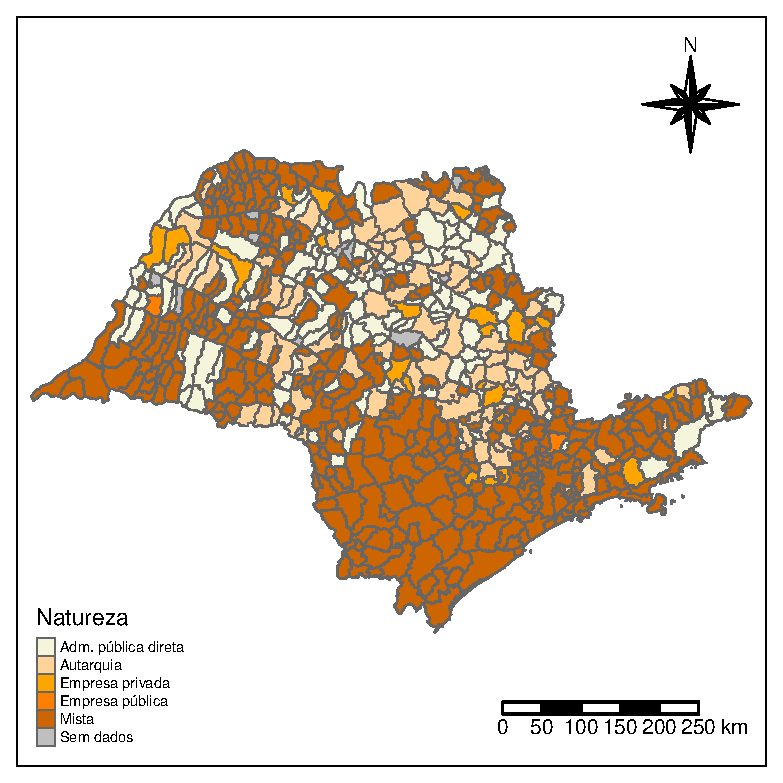
\includegraphics[scale=0.8]{figures/m1.eps}                 
            	\footnotesize \\
            		Fonte: Elaborado pelos autores com dados do SNIS.
    	\label{f:maps15}
	\end{minipage}
\end{figure}





\section{Metodologia}\label{s:metod}


\begin{multicols}{2}
Nesse boletim, analisamos quatro aspectos dos prestadores de serviços de saneamento nos municípios paulistas, considerando a natureza jurídica do prestador. São eles: custos dos serviços para o consumidor final, universalização dos serviços, desempenho financeiro e produtividade, e despesas. Para cada um desses aspectos utilizamos um conjunto de variáveis que refletem cada aspecto que queremos avaliar, isso pode ser visto na Tabela \ref{tab:ind}.
\end{multicols}




\begin{table}[H]\centering
\begin{minipage}{0.9\textwidth}
	\caption{Índicadores utilizados na análise}
	\label{tab:ind}
	\begin{tabular}{l|c}
		\toprule
		\toprule
			Índice & Propósito  \\
			
		\midrule
				IN004 - Tarifa média praticada  &  \multirow{3}{*}{\parbox{6cm}{Verificar o custo dos serviços para o consumidor final}} \\
				IN005 - Tarifa média água       &  \\
				IN006 - Tarifa média esgoto	   &   \\
					                                
		\midrule
				IN015 - Índice de coleta de esgoto & \multirow{3}{*}{\parbox{6cm}{Avaliar a universalização dos serviços de água e esgoto}} \\
				IN016 - Índice de tratamento de esgoto & \\
				IN055 - Índice de atendimento total de água	& \\
													
		\midrule
		
		IN012 - Indicador de desempenho financeiro & \multirow{3}{*}{\parbox{6cm}{Avaliar o desempenho financeiro e a produtividade}} \\
		IN102 - Índice de produtividade de pessoal total & \\		
		IN083 - Duração média dos serviços executados & \\
				
		\midrule
		
		IN008 - Despesa média anual por empregado & \multirow{2}{*}{\parbox{6cm}{Analisar as despesas}} \\
		IN026 - Despesa de exploração por m3 faturado & \\	
		
		\bottomrule
		
	\end{tabular}
\footnotesize \\
	Fonte: Elaborado pelos autores.
\end{minipage}
\end{table}

\begin{multicols}{2}
Para comparar os prestadores de serviços considerando a natureza jurídica utilizamos o Teste de Kruskall-Wallis,  análise de correlação, estatísticas descritivas (média, mediana, máximo, mínimo e desvio padrão) e análise de regressão dos índices apresentados na Tabela \ref{tab:ind}.

O  Teste de Kruskall-Wallis é um teste estatístico não paramétrico utilizado para verificar se amostras de diferentes grupos fazem parte de uma mesma população.
A ideia é verificar se os valores de um determinado índice é diferente quando o agrupamos pela natureza jurídica do prestador de serviço. A hipótese nula é de que os valores de um determinado índice quando agrupados pela natureza jurídica do prestador de serviços fazem parte de uma mesma população. Caso seja aceita podemos dizer que não há diferença entre os grupos em um determinado índice.

Na análise de regressão iremos estimar a seguinte equação:
\begin{equation*}
	\text{IN004} = \alpha_0 +
	 \alpha_1 I_{j} +
	 \sum_{i=1}^{4} \beta_i N_i + 
	 \sum_{i=1}^{4} \gamma_i (N_i \times I_j)
\end{equation*}
onde $\alpha_0$ é o intercepto, $I_j$ é um dos índices da Tabela \ref{tab:ind}, sendo que $j \, \exists \, (1, 2, \cdots, 8)$, e $N_i$ é uma \textit{dummy} que indica a natureza jurídica do prestador de serviços e $i \, \exists \, (1, 2, 3, 4)$. Logo, serão estimadas oito regressões, uma para cada índice da Tabela \ref{tab:ind}, exceto para o IN005 e IN006. 

O intuito é verificar se os prestadores de serviços conseguem reduzir a tarifa média praticada (IN004) dado um aumento na universalização dos serviços, produtividade e despesas. Portanto, na nossa análise iremos focar no coeficiente angular $(\alpha_1 + \gamma_i)$. 

\end{multicols}













 

\section{Resultados}\label{s:resul}

\begin{multicols}{2}

Na Tabela \ref{tab:krusk} apresentamos o Teste de Kruskal-Wallis dos índices que analisamos. A hipótese nula $(H0)$ do teste é de que os valores de um índice específico quando agrupados pela natureza jurídica do prestador de serviços fazem parte de uma mesma população. Nota-se que somente em quatro índice rejeitamos $H0$, ou seja, para esses índices, os grupos fazem parte de populações idênticas não havendo diferenças significativas entre os prestadores de serviços.

\end{multicols}




\begin{table}[H] \centering 
\begin{minipage}{0.3\textwidth}
  \caption{Teste de Kruskal} 
  \label{tab:krusk} 
\begin{tabular}{@{\extracolsep{5pt}} ccc} 
\toprule
\toprule
Índices & \shortstack{Valor p \\ do teste} & H0 \\ 

\midrule

IN004 & $0,00$ & Rejeita \\ 
IN005 & $0,00$ & Rejeita \\ 
IN006 & $0,00$ & Rejeita \\ 
IN015 & $0,08$ & Rejeita \\ 
IN016 & $0,00$ & Rejeita \\ 
IN055 & $0,45$ & Aceita \\ 
IN012 & $0,42$ & Aceita \\ 
IN102 & $0,49$ & Aceita \\ 
IN083 & $0,06$ & Rejeita \\ 
IN008 & $0,49$ & Aceita \\ 
IN026 & $0,00$ & Rejeita \\ 

\bottomrule

\end{tabular} 
	\footnotesize \\
		Fonte: Elaborado pelos autores. 
		Nota: A hipótese nula (H0) é de que os valores dos índices são semelhantes entre as diferentes naturezas jurídicas.
\end{minipage}
\end{table} 


\begin{multicols}{2}

Na Figura \ref{f:corr} temos um correlograma dos índices que estamos analisando. Primeiro vamos discutir as correlações positivas e em seguida as negativas.

Nota-se que as variáveis relacionadas a tarifa média (IN004, IN005, IN006) possuem alta correlação positiva entre si, como já era de se esperar. Os índices relacionados as despesas IN008 e IN026 também possuem alta correlação positiva entre si e com os índices de despesas. Isso indica que quanto maiores as despesas, maior tende a ser as tarifas médias praticadas. 


\end{multicols}


\begin{figure}[H]
        \centering
        	\begin{minipage}{0.55\textwidth}	
                \caption{Correlograma dos índices utilizados no estudo}
                \label{f:corr}
                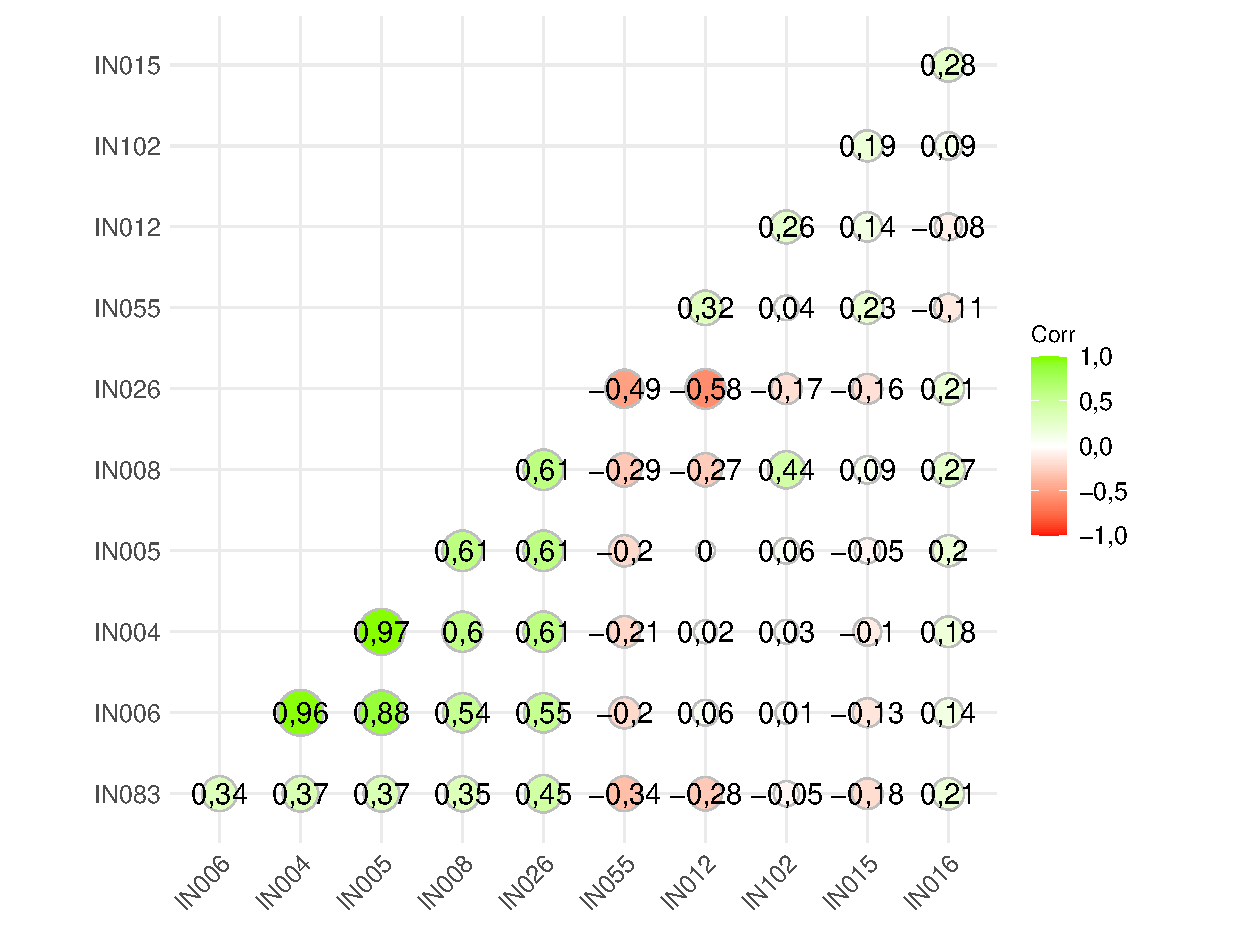
\includegraphics[scale=0.5]{figures/cor.eps}                 
            	\footnotesize \\
            		Fonte: Elaborado pelos autores com dados do SNIS. \\
            		Notas: IN004 - Tarifa média praticada,
				IN005 - Tarifa média água,
				IN006 - Tarifa média esgoto,		
				IN015 - Índice de coleta de esgoto,
				IN016 - Índice de tratamento de esgoto,
				IN055 - Índice de atendimento total de água,	
				IN012 - Indicador de desempenho financeiro,
				IN102 - Índice de produtividade de pessoal total a produtividade,
				IN083 - Duração média dos serviços executados,	
				IN008 - Despesa média anual por empregado,
				IN026 - Despesa de exploração por m3 faturado.   	
	\end{minipage}
\end{figure}







\begin{table}[H] \centering 
\begin{minipage}{1\textwidth}
  \caption{Estatístiscas descritivas dos indicadores utilizados - 2019} 
  \label{tab:desc1} 
  \tiny
    \resizebox{\textwidth}{!}{%
\begin{tabular}{@{\extracolsep{5pt}} cccccc} 
\toprule
\toprule
Índice & Média & Mediana & Máximo & Mínimo & Desvio Padrão \\ 

\midrule

IN004 & $2,50$ & $2,58$ & $4,38$ & $0,93$ & $0,98$ \\ 
IN005 & $2,67$ & $2,77$ & $4,80$ & $1,17$ & $0,93$ \\ 
IN006 & $2,30$ & $2,40$ & $3,68$ & $0,64$ & $1,08$ \\ 
\hline
IN015 & $82,89$ & $86,05$ & $100$ & $50,89$ & $14,70$ \\ 
IN016 & $86,87$ & $100$ & $100$ & $0$ & $30,75$ \\ 
IN055 & $94,75$ & $97,76$ & $100$ & $73,27$ & $6,56$ \\ 
\hline
IN012 & $91,79$ & $88,73$ & $177,52$ & $53,08$ & $26,03$ \\ 
IN102 & $415,32$ & $324,68$ & $1762,47$ & $82,66$ & $309,15$ \\ 
IN083 & $59,97$ & $2,50$ & $420,19$ & $0$ & $93,71$ \\ 
\hline
IN008 & $103.109,40$ & $70.029,21$ & $263.128,60$ & $21.148,81$ & $69.600,69$ \\ 
IN026 & $2,36$ & $2,24$ & $5,46$ & $0,66$ & $1,00$ \\ 

\bottomrule
\end{tabular} }
\footnotesize \\
	Fonte: Elaborado pelos autores com dados do SNIS. \\
	Notas: IN004 - Tarifa média praticada,
	IN005 - Tarifa média água,
	IN006 - Tarifa média esgoto,		
	IN015 - Índice de coleta de esgoto,
	IN016 - Índice de tratamento de esgoto,
	IN055 - Índice de atendimento total de água,	
	IN012 - Indicador de desempenho financeiro,
	IN102 - Índice de produtividade de pessoal total,
	IN083 - Duração média dos serviços executados,	
	IN008 - Despesa média anual por empregado,
	IN026 - Despesa de exploração por m3 faturado.
\end{minipage}
\end{table} 















\begin{table}[H] \centering 
\begin{minipage}{1\textwidth}
  \caption{Média dos índices - 2019} 
  \label{tab:desc2} 
  \small
  \resizebox{\textwidth}{!}{%
\begin{tabular}{@{\extracolsep{5pt}} cccccccc} 
\toprule
\toprule
Índice & \shortstack{Adm. pública \\ direta} & Autarquia & \shortstack{Empresa \\ privada} & \shortstack{Empresa \\ pública} & Mista & \shortstack{Valor Máximo} & \shortstack{Natureza Jur. \\ do valor Máximo} \\ 

\midrule
 
IN004 & $1,41$ & $2,28$ & $2,79$ & $3,40$ & $3,17$ & $3,40$ & Empresa pública \\ 
IN005 & $1,49$ & $2,36$ & $2,99$ & $3,62$ & $3,37$ & $3,62$ & Empresa pública \\ 
IN006 & $0,94$ & $2,17$ & $2,57$ & $3,18$ & $2,94$ & $3,18$ & Empresa pública \\ 
\hline
IN015 & $81,50$ & $86,31$ & $84,78$ & $98$ & $86,50$ & $98$ & Empresa pública \\ 
IN016 & $74,89$ & $77,98$ & $79,90$ & $79,06$ & $94,55$ & $94,55$ & Mista \\ 
IN055 & $90,81$ & $95,99$ & $94,34$ & $94,14$ & $85,23$ & $95,99$ & Autarquia \\ 
\hline
IN012 & $99,63$ & $104,99$ & $110,53$ & $100,94$ & $93,19$ & $110,53$ & Empresa privada \\ 
IN102 & $554,23$ & $306,31$ & $388,25$ & $263,98$ & $715,59$ & $715,59$ & Mista \\ 
IN083 & $4,23$ & $7,44$ & $6,47$ & $0,62$ & $70,15$ & $70,15$ & Mista \\ 
\hline
IN008 & $43.690,26$ & $62.242,77$ & $64.024,46$ & $95.651,97$ & $215.212,00$ & $215.212,00$ & Mista \\ 
IN026 & $1,44$ & $2,06$ & $2,02$ & $3,44$ & $2,91$ & $3,44$ & Empresa pública \\

\bottomrule
\end{tabular} }
\footnotesize \\
	Fonte: Elaborado pelos autores com dados do SNIS. \\
	Notas: IN004 - Tarifa média praticada,
	IN005 - Tarifa média água,
	IN006 - Tarifa média esgoto,		
	IN015 - Índice de coleta de esgoto,
	IN016 - Índice de tratamento de esgoto,
	IN055 - Índice de atendimento total de água,	
	IN012 - Indicador de desempenho financeiro,
	IN102 - Índice de produtividade de pessoal total a produtividade,
	IN083 - Duração média dos serviços executados,	
	IN008 - Despesa média anual por empregado,
	IN026 - Despesa de exploração por m3 faturado.
\end{minipage}
\end{table} 



\begin{table}[H] \centering 
  \caption{Regressão} 
  \label{} 
\begin{tabular}{@{\extracolsep{5pt}}lccc} 
\\[-1.8ex]\hline 
\hline \\[-1.8ex] 
 & \multicolumn{3}{c}{\textit{Dependent variable:}} \\ 
\cline{2-4} 
\\[-1.8ex] & \multicolumn{3}{c}{IN004} \\ 
\\[-1.8ex] & (1) & (2) & (3)\\ 
\hline \\[-1.8ex] 
 IN083 & 0.001 &  &  \\ 
  & (0.001) &  &  \\ 
  & & & \\ 
 IN102 &  & $-$0.0005$^{***}$ &  \\ 
  &  & (0.0001) &  \\ 
  & & & \\ 
 IN055 &  &  & $-$0.004 \\ 
  &  &  & (0.003) \\ 
  & & & \\ 
 Autarquia & 0.707$^{***}$ & 0.752$^{***}$ & 0.886$^{***}$ \\ 
  & (0.187) & (0.157) & (0.155) \\ 
  & & & \\ 
 Empresa privada & 1.418$^{***}$ & 1.305$^{***}$ & 1.395$^{***}$ \\ 
  & (0.289) & (0.254) & (0.255) \\ 
  & & & \\ 
 Empresa pública & 1.991$^{**}$ & 1.856$^{**}$ & 2.003$^{**}$ \\ 
  & (0.827) & (0.800) & (0.804) \\ 
  & & & \\ 
 Mista & 1.693$^{***}$ & 1.838$^{***}$ & 1.742$^{***}$ \\ 
  & (0.139) & (0.114) & (0.114) \\ 
  & & & \\ 
 Constant & 1.408$^{***}$ & 1.667$^{***}$ & 1.748$^{***}$ \\ 
  & (0.114) & (0.125) & (0.324) \\ 
  & & & \\ 
\hline \\[-1.8ex] 
Obs. & 561 & 626 & 626 \\ 
R$^{2}$ & 0.273 & 0.305 & 0.295 \\ 
R$^{2}$ Ajustado & 0.266 & 0.300 & 0.289 \\ 
Residual Std. Error & 1.159  & 1.121  & 1.129  \\ 
F Statistic & 41.638$^{***}$  & 54.469$^{***}$  & 51.883$^{***}$  \\ 
\hline 
\hline \\[-1.8ex] 
\textit{Note:}  & \multicolumn{3}{r}{$^{*}$p$<$0.1; $^{**}$p$<$0.05; $^{***}$p$<$0.01} \\ 
\end{tabular} 
\end{table} 





\section{Conclusão}\label{s:concl}


\begin{appendices}
\setcounter{table}{0}
\setcounter{figure}{0}

\renewcommand{\thetable}{A\arabic{table}}
\renewcommand{\thefigure}{A\arabic{figure}}

\section{}\label{ap1}

\begin{figure}[H]
        \centering
        	\begin{minipage}{0.8\textwidth}	
                \caption{Rigiões Administrativas do estado de São Paulo}
                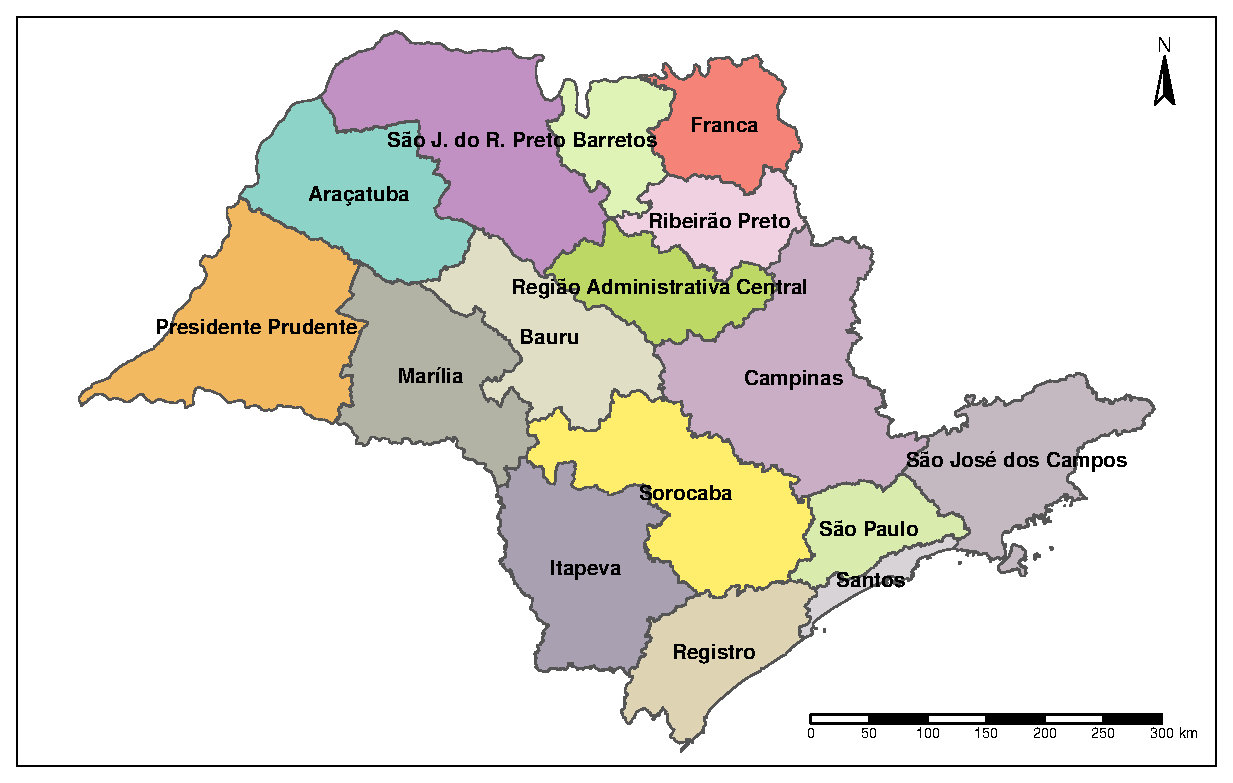
\includegraphics[scale=0.6]{figures/m2.eps}                 
            	\footnotesize \\
            		Fonte: Elaborado pelos autores.
    	\label{f:maps2}
	\end{minipage}
\end{figure}

\end{appendices}




\end{document}


